
\documentclass{standalone}

\usepackage[latin1]{inputenc}
\usepackage{tikz}

% GNUPLOT required
\usepackage{verbatim}

\begin{document}
\pagestyle{empty}

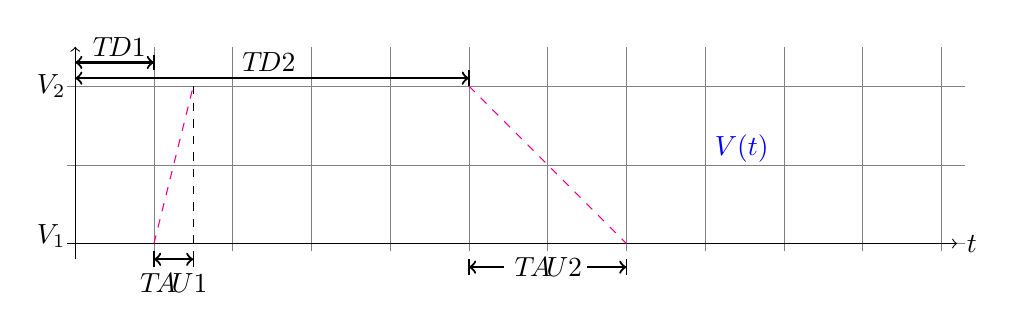
\begin{tikzpicture}[domain=0:11]
    \draw[very thin,color=gray] (-0.1,-0.1) grid (11.3,2.5);
    
    \draw[->] (-0.1,0) -- (11.2,0) node[right] {$t$};
    \draw[->] (0,-.2) -- (0,2.5) node[above] {};
    
    \draw[] (.1,2.5) node[right] {$T\!D1$};
    \draw[thick, <->] (0,2.3) -- (1,2.3) node[] {};
    \draw[semithick, -] (1,2.2) -- (1,2.4) node[] {};

    \draw[] (2,2.3) node[right] {$T\!D2$};
    \draw[thick, <->] (0,2.1) -- (5,2.1) node[] {};
    \draw[semithick, -] (5,2.2) -- (5,2) node[] {};

    \draw[] (.7,-.5) node[right] {$T\!A\!U1$};
    \draw[thick, <->] (1,-.2) -- (1.5,-.2) node[] {};
    \draw[semithick, -] (1,-.1) -- (1,-.3) node[] {};
    \draw[semithick, -] (1.5,-.1) -- (1.5,-.3) node[] {};
    \draw[dashed] (1.5,2) -- (1.5,-.3) node[] {};

    \draw[] (0,2.) node[left] {$V_2$};

    \draw[semithick, -] (5,-.2) -- (5,-.4) node[] {};
    \draw[semithick, -] (7,-.2) -- (7,-0.4) node[] {};
    \draw[thick, <-] (5,-.3) -- (5.45,-.3) node[right] {$T\!A\!U2$};
    \draw[thick, ->] (6.5,-.3) -- (7,-.3) node[] {};
    
    \draw[dashed, color=magenta] (1, 0) -- (1.5,2) node[] {};
    \draw[dashed, color=magenta] (5,2) -- (7,0) node[] {};

    \draw[color=blue, semithick] plot[id=exp1, samples=1000] function{(0+(2-0)*(1-exp(-(x-1)/.5))+(0-2)*(1-exp(-(x-5)/2))*(x>=5 ? 1 : 0))*(x>=1 ? 1 : 0)};


    \draw[] (0,.1) node[left] {$V_1$};


    \draw[color=blue] (8,1.2) node[right] {$V(t)$};

\end{tikzpicture}

\end{document}